\chapter{Introduction}
\label{chap:intro}

In the classical bin packing problem, we are given a set $I$ of items.
Each item $i \in I$ has a size $s(i) \in (0, 1]$ associated with it.
Our goal is to partition $I$ into the minimum number of bins,
such that the sum of sizes of items in each bin is at most 1.
The classical bin packing problem and its generalizations
have diverse applications in computer science and operations research,
like packing goods into trucks, allocating jobs to servers,
allocating memory in computers~\cite{handbook-of-combinopt-bp},
or assigning advertisements to station breaks in television programming,

This work focuses on approximation algorithms for geometric variants
of the classical bin packing problem.
In this chapter, we will first describe the classical bin packing problem
and some of its well-known variants in more detail.
With this context, we will then describe the contributions of this thesis.

\section{Well-Known Packing Problems}

\subsection{Classical Bin Packing}

In the classical bin packing problem, we are given a set $I$ of $n$ items.
Each item $i \in I$ has a size $s(i) \in (0, 1]$ associated with it.
Our goal is to partition $I$ into the minimum number of bins,
such that the sum of sizes of items in each bin is at most 1.
See \cref{fig:1bp-example} for an example.

\begin{figure}[!ht]
\centering
\begin{subfigure}{0.9\textwidth}
    \centering
    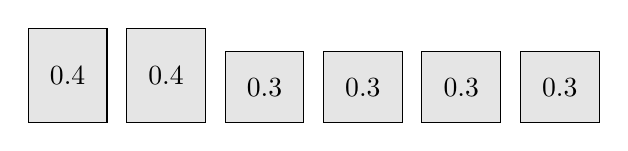
\begin{tikzpicture}[item/.style={fill={black!10},draw}]
\path[item]
    (0,0) rectangle +(1,1.2) node[pos=0.5] {0.4}
    ++(1.25,0) rectangle +(1,1.2) node[pos=0.5] {0.4}
    ++(1.25,0) rectangle +(1,0.9) node[pos=0.5] {0.3}
    ++(1.25,0) rectangle +(1,0.9) node[pos=0.5] {0.3}
    ++(1.25,0) rectangle +(1,0.9) node[pos=0.5] {0.3}
    ++(1.25,0) rectangle +(1,0.9) node[pos=0.5] {0.3};
\end{tikzpicture}

    \caption{A set of six items: two items have size 0.4 and four items have size 0.3.}%
\label{fig:1bp-example:a}
\end{subfigure}
\par\bigskip\bigskip
\begin{subfigure}{0.45\textwidth}
    \centering
    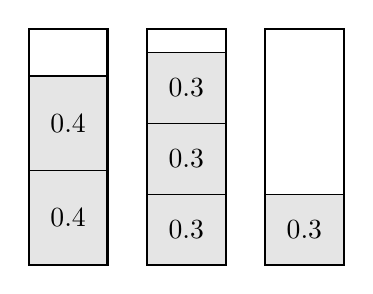
\begin{tikzpicture}[
item/.style={fill={black!10},draw},
bin/.style={draw,thick},
]
\path[item]
    (0.0,0.0) rectangle +(1,1.2) node[pos=0.5] {0.4}
    (0.0,1.2) rectangle +(1,1.2) node[pos=0.5] {0.4}
    (1.5,0.0) rectangle +(1,0.9) node[pos=0.5] {0.3}
    (1.5,0.9) rectangle +(1,0.9) node[pos=0.5] {0.3}
    (1.5,1.8) rectangle +(1,0.9) node[pos=0.5] {0.3}
    (3.0,0.0) rectangle +(1,0.9) node[pos=0.5] {0.3};
\path[bin]
    (0,0) rectangle +(1,3)
    ++(1.5,0) rectangle +(1,3)
    ++(1.5,0) rectangle +(1,3);
\end{tikzpicture}

    \caption{A packing of the items into 3 bins.}
\end{subfigure}
\begin{subfigure}{0.45\textwidth}
    \centering
    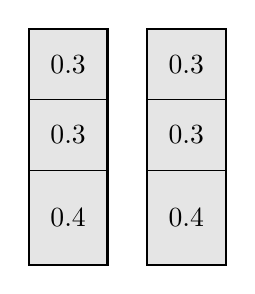
\begin{tikzpicture}[
item/.style={fill={black!10},draw},
bin/.style={draw,thick},
]
\path[item]
    (0.0,0.0) rectangle +(1,1.2) node[pos=0.5] {0.4}
    (0.0,1.2) rectangle +(1,0.9) node[pos=0.5] {0.3}
    (0.0,2.1) rectangle +(1,0.9) node[pos=0.5] {0.3}
    (1.5,0.0) rectangle +(1,1.2) node[pos=0.5] {0.4}
    (1.5,1.2) rectangle +(1,0.9) node[pos=0.5] {0.3}
    (1.5,2.1) rectangle +(1,0.9) node[pos=0.5] {0.3};
\path[bin]
    (0,0) rectangle +(1,3)
    ++(1.5,0) rectangle +(1,3);
\end{tikzpicture}

    \caption{A packing of the items into 2 bins.}
\end{subfigure}
\caption{An example of classical bin packing.
We want to minimize the number of bins, so the packing into 2 bins
is better than the packing into 3 bins.}
\label{fig:1bp-example}
\end{figure}

Classical bin packing is known to be NP-hard.
In fact, deciding whether a set of items can be packed into two bins is NP-complete,
by a simple reduction from the partition problem.
Hence, we look at approximation algorithms.
Let $\opt(I)$ be the minimum number of bins required to pack a set $I$ of items.
An algorithm $\Acal$ is said to be $\alpha$-approximate iff
$\Acal$ requires at most $\alpha\opt(I)$ bins to pack $I$.

Since it is NP-complete to decide whether a set of items can be packed into two bins,
it is NP-hard to obtain a polynomial-time algorithm for bin packing
with approximation ratio less than $3/2$.
(Using the results of D\'osa and Sgall, we can prove that the First-Fit Decreasing algorithm
is $3/2$-approximate~\cite{dosa2013first,dosa2007tight}.)
However, such a reasoning doesn't rule out the existence of an algorithm
that uses $\opt(I) + 1$ bins.
Therefore, we turn our attention to \emph{asymptotic approximation algorithms}.
\begin{definition}[Asymptotic approximation]
A bin packing algorithm $\Acal$ is said to be $\alpha$-asymptotic-approximate iff
$\Acal$ requires at most $\alpha\opt(I) + \beta$ bins to pack $I$
for some value $\beta \in o(\opt(I))$ (usually, $\beta$ is a constant).
$\alpha$ is called the asymptotic approximation ratio (AAR) of $\Acal$.
\end{definition}
\begin{definition}[APTAS]
A bin packing algorithm is called an Asymptotic Polynomial-Time Approximation Scheme (APTAS)
if it accepts a parameter $\eps > 0$ and gives an AAR of $1+\eps$.
The running time for such an algorithm usually increases as $\eps$ decreases.
\end{definition}

For classical bin packing, an APTAS was given by Lueker and Vega~\cite{bp-aptas}.

\subsection{Classical Knapsack}

In the classical knapsack problem, we are given a set $I$ of items.
Each item $i \in I$ has a size $s(i) \in (0, 1]$
and profit $p(i) \in \mathbb{R}_{\ge 0}$ associated with it.
Our goal is to pack the maximum profit subset of $I$ into a bin,
i.e., select a subset $S \subseteq I$ such that
$\sum_{i \in S} s(i) \le 1$ and $\sum_{i \in S} p(i)$ is maximized.
In this problem, the bin is also called \emph{knapsack}.

The classical knapsack problem is NP-hard by a reduction from the subset-sum problem.
Hence, we look at approximation algorithms.
Let $\opt(I)$ be the maximum profit of a subset of $I$ that can be packed into the knapsack.
An algorithm $\Acal$ for the knapsack problem is said to be $\alpha$-approximate iff
the profit of the items packed by $\Acal$ is at least $\opt(I)/\alpha$.

A simple $(1+\eps)$-approximate $O(n^3/\eps)$-time algorithm
exists for this problem~\cite{daa:rounding-dp}.
Lawler improved the running time to $O(n\log(1/\eps) + 1/\eps^4)$~\cite{lawler1979fast}.

\subsection{Geometric Bin Packing}

In the 2-dimensional geometric bin packing problem
(abbreviated as 2D GBP; also called \emph{rectangle bin packing problem}),
we are given a set $I$ of $n$ rectangular items and an infinite supply
of identical rectangular bins.
Our task is to pack the rectangles into the minimum number of bins such that
in each bin, the items don't overlap.
See \cref{fig:2gbp-example} for an example.
For each 2D item $i$, let $w(i)$ denote the width and $h(i)$ denote the height.
Let $a(i) \defeq w(i)h(i)$ be the area of item $i$.

\begin{figure}[htb]
\centering
\ifcsname pGameL\endcsname\else\newlength{\pGameL}\fi
\setlength{\pGameL}{0.325cm}
\begin{tikzpicture}[scale=0.8,
bin/.style={draw,thick},
binGrid/.style={draw,step=1\pGameL,{black!20}},
item/.style={draw},
myarrow/.style={->,>={Stealth},thick},
]
\begin{scope}[yshift=2.1cm]
%\path[binGrid] (0\pGameL, 0\pGameL) grid (19\pGameL, 27\pGameL);
%\path[bin] (0\pGameL, 0\pGameL) rectangle (19\pGameL, 27\pGameL);
\definecolor{currentItemColor}{HTML}{3d7af5}
\path[item,fill=currentItemColor] (1\pGameL, 19\pGameL) rectangle +(7\pGameL, 7\pGameL);
\definecolor{currentItemColor}{HTML}{bb3df5}
\path[item,fill=currentItemColor] (7\pGameL, 0\pGameL) rectangle +(9\pGameL, 6\pGameL);
\definecolor{currentItemColor}{HTML}{813df5}
\path[item,fill=currentItemColor] (0\pGameL, 1\pGameL) rectangle +(6\pGameL, 9\pGameL);
\definecolor{currentItemColor}{HTML}{a23df5}
\path[item,fill=currentItemColor] (7\pGameL, 7\pGameL) rectangle +(8\pGameL, 3\pGameL);
\definecolor{currentItemColor}{HTML}{3de9f5}
\path[item,fill=currentItemColor] (9\pGameL, 19\pGameL) rectangle +(4\pGameL, 7\pGameL);
\definecolor{currentItemColor}{HTML}{d03df5}
\path[item,fill=currentItemColor] (13\pGameL, 11\pGameL) rectangle +(3\pGameL, 7\pGameL);
\definecolor{currentItemColor}{HTML}{f5993d}
\path[item,fill=currentItemColor] (0\pGameL, 11\pGameL) rectangle +(12\pGameL, 2\pGameL);
\definecolor{currentItemColor}{HTML}{f53d40}
\path[item,fill=currentItemColor] (2\pGameL, 16\pGameL) rectangle +(9\pGameL, 2\pGameL);
\definecolor{currentItemColor}{HTML}{3dbef5}
\path[item,fill=currentItemColor] (17\pGameL, 1\pGameL) rectangle +(2\pGameL, 9\pGameL);
\definecolor{currentItemColor}{HTML}{f58a3d}
\path[item,fill=currentItemColor] (17\pGameL, 11\pGameL) rectangle +(2\pGameL, 7\pGameL);
\definecolor{currentItemColor}{HTML}{3dd6f5}
\path[item,fill=currentItemColor] (14\pGameL, 23\pGameL) rectangle +(4\pGameL, 4\pGameL);
\definecolor{currentItemColor}{HTML}{3df5a2}
\path[item,fill=currentItemColor] (14\pGameL, 19\pGameL) rectangle +(5\pGameL, 3\pGameL);
\definecolor{currentItemColor}{HTML}{3df590}
\path[item,fill=currentItemColor] (0\pGameL, 14\pGameL) rectangle +(12\pGameL, 1\pGameL);
\end{scope}
\draw[myarrow] (19\pGameL+0.5cm,6.45cm) -- (10cm-0.5cm,6.45cm);
\begin{scope}[xshift=10cm]
\begin{scope}[yshift=9cm]
%\path[binGrid] (0\pGameL, 0\pGameL) grid (12\pGameL, 12\pGameL);
\definecolor{currentItemColor}{HTML}{813df5}
\path[item,fill=currentItemColor] (0\pGameL, 3\pGameL) rectangle +(6\pGameL, 9\pGameL);
\definecolor{currentItemColor}{HTML}{d03df5}
\path[item,fill=currentItemColor] (8\pGameL, 3\pGameL) rectangle +(3\pGameL, 7\pGameL);
\definecolor{currentItemColor}{HTML}{f5993d}
\path[item,fill=currentItemColor] (0\pGameL, 0\pGameL) rectangle +(12\pGameL, 2\pGameL);
\definecolor{currentItemColor}{HTML}{3dbef5}
\path[item,fill=currentItemColor] (6\pGameL, 3\pGameL) rectangle +(2\pGameL, 9\pGameL);
\definecolor{currentItemColor}{HTML}{3df590}
\path[item,fill=currentItemColor] (0\pGameL, 2\pGameL) rectangle +(12\pGameL, 1\pGameL);
\path[bin] (0\pGameL, 0\pGameL) rectangle (12\pGameL, 12\pGameL);
\end{scope}
\begin{scope}[yshift=4.5cm]
%\path[binGrid] (0\pGameL, 0\pGameL) grid (12\pGameL, 12\pGameL);
\definecolor{currentItemColor}{HTML}{bb3df5}
\path[item,fill=currentItemColor] (0\pGameL, 0\pGameL) rectangle +(9\pGameL, 6\pGameL);
\definecolor{currentItemColor}{HTML}{a23df5}
\path[item,fill=currentItemColor] (0\pGameL, 8\pGameL) rectangle +(8\pGameL, 3\pGameL);
\definecolor{currentItemColor}{HTML}{f53d40}
\path[item,fill=currentItemColor] (0\pGameL, 6\pGameL) rectangle +(9\pGameL, 2\pGameL);
\definecolor{currentItemColor}{HTML}{f58a3d}
\path[item,fill=currentItemColor] (9\pGameL, 0\pGameL) rectangle +(2\pGameL, 7\pGameL);
\path[bin] (0\pGameL, 0\pGameL) rectangle (12\pGameL, 12\pGameL);
\end{scope}
\begin{scope}
%\path[binGrid] (0\pGameL, 0\pGameL) grid (12\pGameL, 12\pGameL);
\definecolor{currentItemColor}{HTML}{3d7af5}
\path[item,fill=currentItemColor] (0\pGameL, 0\pGameL) rectangle +(7\pGameL, 7\pGameL);
\definecolor{currentItemColor}{HTML}{3de9f5}
\path[item,fill=currentItemColor] (7\pGameL, 0\pGameL) rectangle +(4\pGameL, 7\pGameL);
\definecolor{currentItemColor}{HTML}{3dd6f5}
\path[item,fill=currentItemColor] (0\pGameL, 7\pGameL) rectangle +(4\pGameL, 4\pGameL);
\definecolor{currentItemColor}{HTML}{3df5a2}
\path[item,fill=currentItemColor] (4\pGameL, 7\pGameL) rectangle +(5\pGameL, 3\pGameL);
\path[bin] (0\pGameL, 0\pGameL) rectangle (12\pGameL, 12\pGameL);
\end{scope}
\end{scope}
\end{tikzpicture}

\caption{Packing 13 rectangles into 3 bins (without rotation).}
\label{fig:2gbp-example}
\end{figure}

There are two commonly-studied versions of 2D GBP.
In the non-rotational version, rotating the items is forbidden.
In the rotational version, the items can be rotated by $90^{\circ}$.
In both versions, the items and bins are oriented parallel to the coordinate axes.
See \cref{fig:rot-vs-nonrot} for an example.
Note that if all items have width equal to 1, then 2D GBP reduces to
the classical bin packing problem.

\begin{figure}[htb]
\centering
\begin{subfigure}{0.5\textwidth}
    \centering
    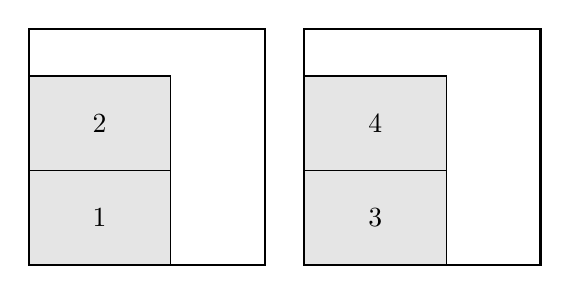
\begin{tikzpicture}[
item/.style={fill={black!10},draw},
bin/.style={draw,thick},
]
\path[item]
    (0.0,0.0) rectangle +(1.8,1.2) node[pos=0.5] {1}
    (0.0,1.2) rectangle +(1.8,1.2) node[pos=0.5] {2}
    (3.5,0.0) rectangle +(1.8,1.2) node[pos=0.5] {3}
    (3.5,1.2) rectangle +(1.8,1.2) node[pos=0.5] {4};
\path[bin]
    (0,0) rectangle +(3,3)
    ++(3.5,0) rectangle +(3,3);
\end{tikzpicture}

    \caption{Packing without item rotation}
\end{subfigure}
\begin{subfigure}{0.4\textwidth}
    \centering
    \begin{tikzpicture}[
item/.style={fill={textColor!10!bgColor},draw},
bin/.style={draw,thick},
]
\path[item]
    (0.0,0.0) rectangle +(1.8,1.2) node[pos=0.5] {1}
    (1.8,0.0) rectangle +(1.2,1.8) node[pos=0.5] {2}
    (0.0,1.2) rectangle +(1.2,1.8) node[pos=0.5] {3}
    (1.2,1.8) rectangle +(1.8,1.2) node[pos=0.5] {4};
\path[bin]
    (0,0) rectangle +(3,3);
\end{tikzpicture}

    \caption{Packing with item rotation}
\end{subfigure}
\caption{Packing 4 rectangular items, each of width 0.6 and height 0.4,
into square bins of side length 1.
Allowing rotation decreases the minimum number of bins needed to pack these items.}
\label{fig:rot-vs-nonrot}
\end{figure}

2D GBP finds applications in the wood-cutting, metal-cutting, paper and cloth industries,
where rectangular pieces need to be cut out of standard-sized sheets,
and item rotations are usually allowed.
Non-rotational 2D GBP can be used for placing advertisements on web pages and newspapers.

The problem can be extended to three dimensions (3D GBP),
where the bins and items are cuboids.
Since a cuboid can have 6 possible orientations (see \cref{fig:3d-orients}), there can be
many versions of 3D GBP depending on which orientations of items are allowed.
3D GBP can be used to pack boxes into shipping containers.
Here the boxes can usually be rotated in any way, but there are exceptions:
for example, some boxes may need to be kept upright due to fragile contents inside.
Such boxes can only be rotated around the vertical axis.

\begin{figure}[htb]
\centering
\tikzset{pics/cuboid/.style args={#1,#2,#3}{code={
\fill[black!15] (0,0,#3) -- ++(#1,0,0) -- ++(0,#2,0) -- ++(-#1,0,0) -- cycle;
\fill[black!30] (0,0,0) -- +(#1,0,0) -- +(#1,0,#3) -- +(0,0,#3) -- cycle;
%\fill[black!45] (#1,0,0) -- ++(0,#2,0) -- ++(0,0,#3) -- ++(0,-#2,0) -- cycle;
\fill[black!45] (0,0,0) -- ++(0,0,#3) -- ++(0,#2,0) -- ++(0,0,-#3) -- cycle;
}}}
\begin{tikzpicture}[isometric view]

\begin{scope}[xshift=0cm]
\pic{cuboid={0.4,0.8,1.6}};
\end{scope}

\begin{scope}[xshift=1.5cm]
\pic{cuboid={0.8,0.4,1.6}};
\end{scope}

\begin{scope}[xshift=4cm,yshift=0.1cm]
\pic{cuboid={0.4,1.6,0.8}};
\end{scope}

\begin{scope}[xshift=5.5cm,yshift=0.1cm]
\pic{cuboid={1.6,0.4,0.8}};
\end{scope}

\begin{scope}[xshift=8.5cm,yshift=0.2cm]
\pic{cuboid={0.8,1.6,0.4}};
\end{scope}

\begin{scope}[xshift=10.5cm,yshift=0.2cm]
\pic{cuboid={1.6,0.8,0.4}};
\end{scope}
\end{tikzpicture}

\caption{All six orientations of a cuboid of dimensions 0.2, 0.4 and 0.8.}
\label{fig:3d-orients}
\end{figure}

We can extend 2D and 3D GBP to even higher dimensions.
In $d$D GBP ($d \ge 1$), items and bins are $d$D cuboids.
A $d$D cuboid is defined as the cross-product of $d$ intervals from the real line.
A cube is a cuboid that has the same length in each dimension.
For example, a $d$D cube of side length 1 is the set $[0, 1]^d$.
Note that 1D GBP is the classical bin packing problem.

In the non-rotational version of $d$D GBP, we can assume \wLoG{} that
the bin is a cube of side length 1.
This is because we can scale the dimensions of the bins and items by the same factor.
Note that this assumption doesn't hold for the rotational version.

For 2D GBP, the algorithm by Bansal and Khan~\cite{bansal2014binpacking}
gives the best-known AAR of $1 + \ln(1.5) + \eps \approx 1.40547 + \eps$.
An APTAS cannot exist for 2D GBP unless P = NP~\cite{bansal2006bin,chlebik2009hardness}.
For non-rotational $d$D GBP where $d \ge 3$, the algorithm by Caprara~\cite{caprara2008}
gives the best-known AAR of roughly $T_{\infty}^{d-1}$, where $T_{\infty} \approx 1.69103$.

\subsection{Guillotine-Separable Geometric Bin Packing}

In many practical cases of 2D GBP, there are additional constraints on
how items can be packed into bins, like in the
\emph{two-dimensional guillotine-separable geometric bin packing problem} (2D GuillBP).

\begin{definition}
A packing of rectangles into a bin is said to be
\emph{$k$-stage guillotine-separable} or \emph{$k$-stage guillotinable}
iff we can separate all the items in the bin using at most $k$ stages of end-to-end cuts
(also called \emph{guillotine cuts}), where in each stage,
all cuts are parallel to the $x$-axis or all cuts are parallel to the $y$-axis.
A packing of rectangles into a bin is said to be \emph{guillotine-separable}
or \emph{guillotinable} iff it is $k$-stage guillotinable for some $k$.
\end{definition}

See \cref{fig:guill-example} for an example of 3-stage guillotinable packing
and \cref{fig:non-guill-examples} for examples of non-guillotinable packing.

\begin{figure}[htb]
\centering
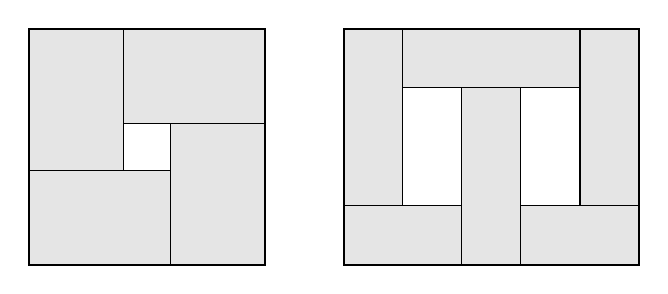
\begin{tikzpicture}[
item/.style={fill={black!10},draw},
bin/.style={draw,thick},
]
\path[item]
    (0.0,0.0) rectangle +(1.8,1.2)
    (1.8,0.0) rectangle +(1.2,1.8)
    (0.0,1.2) rectangle +(1.2,1.8)
    (1.2,1.8) rectangle +(1.8,1.2);
\path[bin] (0,0) rectangle +(3,3);
\begin{scope}[shift={(4cm,0cm)},scale=1.25]
\path[item]
    (0.0,0.0) rectangle +(1.2,0.6)
    (1.8,0.0) rectangle +(1.2,0.6)
    (0.0,0.6) rectangle +(0.6,1.8)
    (2.4,0.6) rectangle +(0.6,1.8)
    (1.2,0.0) rectangle +(0.6,1.8)
    (0.6,1.8) rectangle +(1.8,0.6);
\path[bin] (0,0) rectangle +(3,2.4);
\end{scope}
\end{tikzpicture}

\caption{Two bins that are not guillotinable.}
\label{fig:non-guill-examples}
\end{figure}
\begin{figure}[htb]
\centering
\tikzset{pics/mypic/.style args={#1,#2,#3}{code={
\begin{scope}
    \begin{scope}
        \begin{scope}
            \path[item] (0, 0) rectangle +(0.8, 2.4);
            \path[bin3] (0, 0) rectangle +(0.8, 2.4);
        \end{scope}
        \begin{scope}[xshift={#3cm}]
            \path[item] (0.8, 0) rectangle +(0.6, 2.4);
            \path[bin3] (0.8, 0) rectangle +(0.6, 2.4);
        \end{scope}
        \begin{scope}[xshift={2*#3cm}]
            \path[item] (1.4, 0) rectangle +(0.8, 2);
            \path[bin3] (1.4, 0) rectangle +(1, 2.4);
        \end{scope}
        \path[bin2] (0, 0) rectangle +(2.4, 2.4);
        \path[cutline2] (0.8, -0.2) -- (0.8, 2.6);
        \path[cutline2] (1.4, -0.2) -- (1.4, 2.6);
    \end{scope}
    \begin{scope}[yshift={#2cm}]
        \begin{scope}
            \path[item] (0, 2.4) rectangle +(1.1, 1.6);
            \path[bin3] (0, 2.4) rectangle +(1.1, 1.6);
        \end{scope}
        \begin{scope}[xshift={#3cm}]
            \path[item] (1.1, 2.4) rectangle +(1.3, 1.4);
            \path[bin3] (1.1, 2.4) rectangle +(1.3, 1.6);
        \end{scope}
        \path[bin2] (0, 2.4) rectangle +(2.4, 1.6);
        \path[cutline2] (1.1, 2.2) -- (1.1, 4.2);
    \end{scope}
    \path[cutline1] (-0.2, 2.4) -- (2.6, 2.4);
    \path[bin1] (0, 0) rectangle +(2.4, 4);
\end{scope}
\begin{scope}[xshift={#1cm}]
    \begin{scope}
        \begin{scope}
            \path[item] (2.4, 0) rectangle +(0.8, 2.8);
            \path[bin3] (2.4, 0) rectangle +(0.8, 3.2);
        \end{scope}
        \begin{scope}[xshift={#3cm}]
            \path[item] (3.2, 0) rectangle +(0.8, 3.2);
            \path[bin3] (3.2, 0) rectangle +(0.8, 3.2);
        \end{scope}
        \path[bin2] (2.4, 0) rectangle +(1.6, 3.2);
        \path[cutline2] (3.2, -0.2) -- (3.2, 3.4);
    \end{scope}
    \begin{scope}[yshift={#2cm}]
        \path[item] (2.4, 3.2) rectangle +(1.6, 0.6);
        \path[bin2,bin3] (2.4, 3.2) rectangle +(1.6, 0.8);
    \end{scope}
    \path[bin1] (2.4, 0) rectangle +(1.6, 4);
    \path[cutline1] (2.2, 3.2) -- (4.2, 3.2);
\end{scope}
\path[bin0] (0, 0) rectangle +(4, 4);
\path[cutline0] (2.4, -0.2) -- (2.4, 4.2);
}}}
\begin{tikzpicture}[
item/.style={fill={black!10},draw},
myarrow/.style={->,>={Stealth},thick},
bin/.style={draw,thick},
cutline/.style={draw={black!50!red},densely dashed,line width=1.1pt},
bin0/.style={},
bin1/.style={},
bin2/.style={},
bin3/.style={},
cutline0/.style={},
cutline1/.style={},
cutline2/.style={},
]
\begin{scope}[bin0/.style=bin,cutline0/.style=cutline]
    \pic[yscale=-1]{mypic={0,0,0}};
    \node[rotate=90,transform shape] at (2.42,-4.35) {\large\ding{34}};
\end{scope}
\draw[myarrow] (5,-2) -> (8,-2);
\begin{scope}[xshift=9.5cm,bin1/.style=bin,cutline1/.style=cutline]
    \pic[yscale=-1]{mypic={1,0,0}};
    \node[transform shape] at (-0.4,-2.42) {\large\ding{34}};
    \node[xscale=-1,transform shape] at (5.4,-3.22) {\large\ding{34}};
\end{scope}
\draw[myarrow] (12.1,-4.5) -> (12.1,-6);
\begin{scope}[shift={(9.5cm,-7cm)},bin2/.style=bin,cutline2/.style=cutline]
    \pic[yscale=-1]{mypic={1,0.5,0}};
    \node[yscale=-1,rotate=90,transform shape] at (0.82,0.4) {\large\ding{34}};
    \node[yscale=-1,rotate=90,transform shape] at (1.42,0.4) {\large\ding{34}};
    \node[yscale=-1,rotate=90,transform shape] at (4.22,0.4) {\large\ding{34}};
    \node[rotate=90,transform shape] at (1.12,-4.9) {\large\ding{34}};
\end{scope}
\draw[myarrow] (8.5,-9.5) -> (6.5,-9.5);
\begin{scope}[yshift=-7cm,bin3/.style=bin]
    \pic[yscale=-1]{mypic={1.2,0.5,0.4}};
\end{scope}
\end{tikzpicture}

\caption{Separating items using 3 stages of guillotine cuts.}
\label{fig:guill-example}
\end{figure}

2D GuillBP is a variant of 2D GBP where we are given a set $I$ of rectangles and
our task is to pack them into the minimum number of bins such that each bin is guillotinable.
Similarly, in the $k$-stage 2D bin packing problem, we have to pack a set of rectangles
into the minimum number of bins such that each bin is $k$-stage guillotinable.

2D GuillBP is relevant in sheet-cutting
industries~\cite{mchale1999cutting,puchinger2004solving,schneider1988trim},
where cutting machines can only make guillotine cuts.
Guillotine cuts simplify the design and programming of cutting machines
and reduce their operational cost, which is important if
the raw material being cut is relatively inexpensive.

Unlike 2D GBP, which is APX-hard, an APTAS is known for 2D GuillBP~\cite{bansal2005tale}.

\subsection{Vector Bin Packing}

In the $d$-dimensional vector bin packing problem ($d$D VBP),
we are given a set $I$ of $d$-dimensional vectors,
and our task is to partition the vectors into bins such that in each bin,
the sum of the vectors in that bin have $\ell_\infty$-norm at most 1.
Formally, let $I \defeq \{v^{(1)}, v^{(2)}, \ldots, v^{(n)}\}$ be the items,
where $v^{(i)} \in (0, 1]^d$ for each $i$.
Then we have to partition the vectors into bins such that in each bin $B$,
$\sum_{v \in B} v_j \le 1$ for each $j \in \{1, 2, \ldots, d\}$.

\begin{figure}[htb]
\centering
\begin{subfigure}{0.45\textwidth}
    \centering
    \begin{tikzpicture}[
item/.style={->,>={Stealth},ultra thick},
]
\definecolor{myColor}{HTML}{00b0f0}
\draw[myColor,item] (0,0) -- +(0.3,1.5);
\definecolor{myColor}{HTML}{bf9000}
\draw[myColor,item] (0.8,0) -- +(1.2,2.4);
\definecolor{myColor}{HTML}{92d050}
\draw[myColor,item] (1.7,0) -- +(0.9,0.9);
\definecolor{myColor}{HTML}{c00000}
\draw[myColor,item] (2.7,0) -- +(1.5,0.6);
\definecolor{myColor}{HTML}{7030a0}
\draw[myColor,item] (4.5,0) -- +(1.5,0.3);
\end{tikzpicture}

    \caption{Five 2D vectors.}
\end{subfigure}
\begin{subfigure}{0.54\textwidth}
    \centering
    \begin{tikzpicture}[
item/.style={->,>={Stealth},ultra thick},
bin/.style={draw,thick},
]
\definecolor{myColor}{HTML}{c00000}
\draw[myColor,item] (0,0) -- +(1.5,0.6);
\definecolor{myColor}{HTML}{bf9000}
\draw[myColor,item] (1.5,0.6) -- +(1.2,2.4);
\path[bin] (0,0) rectangle (3,3);
\begin{scope}[xshift=3.5cm]
\definecolor{myColor}{HTML}{00b0f0}
\draw[myColor,item] (0,0) -- +(0.3,1.5);
\definecolor{myColor}{HTML}{92d050}
\draw[myColor,item] (0.3,1.5) -- +(0.9,0.9);
\definecolor{myColor}{HTML}{7030a0}
\draw[myColor,item] (1.2,2.4) -- +(1.5,0.3);
\path[bin] (0,0) rectangle (3,3);
\end{scope}
\end{tikzpicture}

    \caption{Packing the vectors into two bins.
    A set of 2D vectors lies in a bin iff their sum
    lies inside a square of side length 1.}
\end{subfigure}
\caption{Packing five 2D vectors into two bins.}
\label{fig:2vbp-example}
\end{figure}

$d$D VBP has applications in resource allocation problems.
Consider a set of tasks, each of which have a $d$ resource requirements.
The resources could be CPU time, memory, disk IO, network IO, etc.
We have to assign these tasks to the minimum number of servers,
where each server has a capacity on each resource.
This is an example of $d$D VBP, where the tasks are items and servers are bins.

For $d$D VBP, the best-known AAR is $\ln d + O(1)$~\cite{rna,bansal2016improved}.
For 2D VBP, the best-known AAR is
$1 + \ln(1.5) + \eps \approx 1.40547 + \eps$~\cite{bansal2016improved}.

\section{Contributions of This Thesis}

In this thesis, we address the following four problems related to geometric bin packing.

\subsection{Generalized Multidimensional Bin Packing}

Geometric packing and vector packing are well-studied generalizations of
the classical bin packing problem.
% \cref{fig:geom-vec-diff} in \cref{app:figs} illustrates the difference between
% geometric packing and vector packing.
However, often in practice, we encounter a mixture of geometric and vector constraints.
Consider the following airlines cargo problem~\cite{paquay2016mixed}:
We have boxes to load in an airline cargo container.
In addition to the geometric constraint that all the boxes must fit within the container,
we also have a constraint that the total weight of the loaded boxes
should be within a specified capacity. Thus, in this problem,
three dimensions are geometric and the weight is a vector constraint.

Weight has been an important constraint to consider for packing in logistics and supply chain
management, e.g., cranes and other equipment can be damaged by the bins being too heavy,
or by a skewed weight distribution~\cite{alonso2017mathematical}.
While the container loading problems mostly consider packing items inside a container,
the container stowage planning problem considers the stacking of the containers
onto and off cargo ships~\cite{monaco2014terminal}.
Even when different cargoes are packed into a fleet of aircraft for transport,
one needs the individual cargoes to be not too heavy to ensure stability
and less fuel consumption~\cite{amiouny1992balanced}.
Similar problems find applications in vehicle routing
with loading constraints~\cite{bortfeldt2013constraints}.
Many practical heuristics~\cite{sorset2019heuristic,taylor2017three}
have been proposed for these kinds of problems.
Several companies (such as Driw, Boxify, Freightcom) and practical packages~\cite{yang2017gbp}
have considered the problem. In many cases, we also want to ensure a limit on other attributes,
such as the amount of magnetism, radioactivity, or toxicity.
Each of these properties can be considered as additional vector dimensions.

Such multidimensional packing problems are also getting attention due to their
connections with fair resource allocation~\cite{fairknap}.
In recent years, a considerable amount of research has focused on
group fairness~\cite{JosephKMR16,TsangWRTZ19} such that the algorithms are
not biased towards (or against) some groups or categories.
One such notion of fairness is \emph{restricted dominance}~\cite{BeraCFN19},
which upper bounds the number (or size) of items from a category.
These different categories can be considered as dimensions.
E.g., in a container packing problem for flood relief,
one needs to ensure that the money spent on a container is fairly distributed among
different types of items (such as medicine, food, garments).
Hence, for each category, there is an upper bound on the value that can go into a container.

Formally, we are given $n$ items $I\defeq\{1, 2, \dots, n\}$
that are \geomvecdim{$d_g$}{$d_v$}, i.e., item $i$ is a
$d_g$-dimensional cuboid of lengths $\ell_1(i), \ell_2(i), \ldots, \ell_{d_g}(i)$
and has $d_v$ non-negative weights $v_1(i), v_2(i), \ldots, v_{d_v}(i)$.
A \geomvecdim{$d_g$}{$d_v$} bin is a $d_g$-dimensional cuboid of length 1
in each geometric dimension and weight capacity 1 in each of the $d_v$ vector dimensions.
A feasible packing of items into a bin is a packing where items are packed parallel to the axes
without overlapping, and for all $j \in [d_v]$,
the sum of the $j\Th$ weight-dimension of the items in the bin is at most 1.
In the \geomvec{$d_g$}{$d_v$} bin packing problem (BP),
we have to feasibly pack all items into the minimum number of bins.
In the \geomvec{$d_g$}{$d_v$} knapsack problem (KS),
each item $i$ also has an associated nonnegative profit $p(i)$,
and we have to feasibly pack a maximum-profit subset of the items into a single bin
(also called \emph{knapsack}).
\geomvec{$d_g$}{$d_v$} packing problems generalize both $d_g$-dimensional geometric packing
(when $d_v=0$) and $d_v$-dimensional vector packing (when $d_g=0$).
Already for vector packing, if $d_v$ is part of the input, there is an approximation
hardness of ${d_v}^{1-\eps}$ unless NP=ZPP~\cite{bansal2016improved}.
Thus, throughout the paper we assume both $d_g, d_v$ to be constants.

\subsubsection{Our Results}

We study the first approximation algorithms for general \geomvec{$d_g$}{$d_v$} BP,
with a focus on $d_g = 2$.
We give two simple algorithms for \geomvec{2}{$d$} BP, called $\simplePack$
and $\betterSimplePack$, having AARs of $6(d+1)$ and $3(1+\ln(d+1))+\eps$,
respectively, for any $\eps > 0$.
For $d = 1$, $\betterSimplePack$'s AAR improves to $\approx 4.21640 + \eps$.

Next, we modify the Round-and-Approx (R\&A) framework~\cite{rna,bansal2014binpacking}
so that it works for \geomvec{$d_g$}{$d_v$} BP.
We combine R\&A with the $\simplePack$ algorithm to get an AAR of
$2(1 + \ln(3(d+1))) + \eps$ for \geomvec{2}{$d$} BP.
This improves upon the AAR of $\betterSimplePack$ for $d \ge 3$.

Next, we obtain a more sophisticated algorithm for \geomvec{2}{$d$} BP, called $\cbPack$,
that fits into the R\&A framework and has an even better AAR.
\begin{theorem}
\label{thm:2-d-gvbp}
For any $\eps > 0$, there is a polynomial-time algorithm for \geomvec{2}{$d$} BP,
called $\cbPack$, having AAR $2(1+\ln((d+4)/2))+\eps$
(improves to $2(1+\ln((d+3)/2))+\eps$ when items can be rotated by $90^{\circ}$).
For $d=1$, the AAR improves to $2(1+\ln(19/12))+\eps$ $\approx 2.919 + \eps$
(further improves to $2(1+\ln(3/2))+\eps$ $\approx 2.811 + \eps$ when items can be rotated).
\end{theorem}

\begin{table}[!ht]
\centering
\caption{Comparison of asymptotic approximation ratios
of our algorithms for \geomvec{2}{$d$} BP.}
\begin{tabular}{lcc}
\toprule Algorithm
    & AAR for \geomvec{2}{$d$} BP
    & AAR for \geomvec{2}{1} BP
\\ \midrule $\simplePack$
    & $6(d+1)$
    & $12$
    % & \cref{sec:simple-algos}
\\[\defaultaddspace] $\betterSimplePack$
    & $3(1 + \ln(d+1)) + \eps$
    & $3(1 + \ln(3/2)) + \eps \approx 4.216+\eps$
    % & \cref{sec:simple-algos}
%\\ \hline \parbox[l][2em][c]{14em}{$\simplePack$ with R\&A}
\\[\defaultaddspace] $\simplePack$ with R\&A
    & $2(1 + \ln(3(d+1))) + \eps$
    & $2(1 + \ln 6) + \eps$ $\approx 5.5835+\eps$
    %& \cref{sec:rna:simple-pack}
\\[\defaultaddspace] $\cbPack$ (without rotation)
    & {$2(1+\ln(\frac{d+4}{2})) + \eps$}
    & $2(1+\ln(19/12))+\eps$ $\approx 2.919+\eps$
    %& \cref{thm:2-d-gvbp}
\\[\defaultaddspace] $\cbPack$ (with rotation)
    & ${2(1+\ln(\frac{d+3}{2})) + \eps}$
    & $2(1+\ln(3/2))+\eps$ $\approx 2.811+\eps$
    %& \cref{thm:2-d-gvbp}
\\ \bottomrule
\end{tabular}
\label{table:gvbp-aar}
\end{table}

We also show how to extend $\simplePack$ and $\betterSimplePack$ to \geomvec{$d_g$}{$d_v$} BP
to obtain AARs $2b(d_v+1)$ and $b(1 + \ln(d_v + 1) + \eps)$, respectively,
where $b \defeq 4^{d_g} + 2^{d_g}$.
We also give a similar algorithm for \geomvec{$d_g$}{$d_v$} KS
having approximation ratio $b(1+\eps)$.

One of our main contributions is the enhancement of
the R\&A framework~\cite{rna,bansal2014binpacking} to a wider class of algorithms.
The R\&A framework is a simple but powerful technique,
originally given by Bansal, Caprara and Sviridenko~\cite{rna},
to improve the AAR of a bin packing algorithm by combining it with
randomized rounding of a linear program.
R\&A may have the potential to improve the AARs of several packing problems,
but its applicability is limited because
it only works with \emph{subset-oblivious} bin packing algorithms,
and proving that an algorithm is subset-oblivious is difficult.

Bansal and Khan~\cite{bansal2014binpacking} partially removed this limitation
by proving that a large class of algorithms for geometric and vector bin packing,
called \emph{Rounding-based} algorithms, is subset-oblivious.
We make further improvements on this front by showing that an even larger class
of algorithms is subset-oblivious.
This class includes some of our algorithms for \geomvec{$d_g$}{$d_v$} BP,
like $\simplePack$ and $\cbPack$.
We expect that our progress will help in better understanding the power of R\&A
and extending it to other set-cover type problems,
like round-SAP and round-UFP~\cite{ElbassioniGGKNP12}.

\subsection{Harmonic Algorithms for \texorpdfstring{$d$}{d}D GBP with Rotations}

In his seminal paper, Caprara~\cite{caprara2008} devised a polynomial-time algorithm
for non-rotational $d$D GBP called $\hdhk$ (Harmonic Decreasing Height),
where $k \in \mathbb{Z}$ is a parameter to the algorithm.
$\hdhk$ has AAR equal to $T_k^{d-1}$,
where $T_k$ is a decreasing function of $k$ and
$T_{\infty} \defeq \lim_{k \to \infty} T_k \approx 1.69103$.
The algorithm $\hdhk$ is based on an extension of the harmonic algorithm~\cite{leelee}
for classical bin packing.
For $d \ge 3$ and large $k$, $\hdhk$ has the best AAR
among all known algorithms for $d$D GBP.

A limitation of $\hdhk$ is that it does not allow rotation of items.
This is in contrast to some real-world problems,
like packing boxes into shipping containers ($d=3$),
where items can often be rotated orthogonally,
i.e., $90^{\circ}$ rotation around all or a subset of axes.

Furthermore, known algorithms for rotational 3D GBP have a significantly larger AAR
than what the $\hdhk$ algorithm gives for non-rotational 3D GBP.
When items can be rotated about all axes,
Miyazawa and Wakabayashi~\cite{miyazawa2009three} gave a
4.89-asymptotic-approximation algorithm.
Epstein and van Stee~\cite{epstein2006side} improved the AAR to
4.5 when the base of the bin is a square.
On the other hand, $\hdhk$ gives an AAR of roughly
$T_{\infty}^2 \approx 2.85958$ for large $k$.

Orientation constraints may sometimes limit the vertical orientation of a box to one dimension
(e.g., some items require a face labeled `This side up' to always be one top)
or to two (of three) dimensions
(e.g., long but low and narrow box should not be placed on its smallest surface).
These constraints are introduced to deter goods
and packaging from being damaged and to ensure the stability of the load.
Current algorithms for 3D GBP either allow rotating all items along the same set of axes
or don't allow rotating any item, i.e., they enforce the same
orientation constraints over all items in the input.

\begin{comment}
The state-of-the-art algorithms for 2D GBP allow rotating items,
but they assume that the bin is square, which is often not true in practice.
For $d > 3$, there are no known approximation algorithms for $d$D GBP
when items can be rotated.
\end{comment}

We address these issues by giving algorithms for $d$D GBP
that are similar to $\hdhk$ but allow items to be rotated
and allow orientation constraints to vary across items.
We first give a fast and simple algorithm called $\fhk$ that has an AAR of $T_k^d$.
We next give a more sophisticated algorithm called $\hgapk$
that has an AAR of $T_k^{d-1}(1+\eps)$.

\subsubsection{Multiple-Choice Packing}

$\fhk$ and $\hgapk$ can be extended to work for the $d$D multiple-choice
geometric bin packing problem ($d$MCBP), which we will describe now.
$d$MCBP generalizes both the rotational and non-rotational versions of $d$D GBP.
It also captures the concept of variable orientation constraints across items.
This perspective will help us design algorithms for the rotational case.

In $d$MCBP, we are given a set $\Ical = \{I_1, I_2, \ldots, I_n\}$,
where for each $j$, $I_j$ is a set of items, henceforth called an {\em itemset}.
We have to pick exactly one item from each itemset and pack those items
into the minimum number of bins.

We can model rotation using multiple-choice packing:
Given a set $I$ of items, for each item $i \in I$,
create an itemset $I_i$ that contains all allowed orientations of $i$.
Then the optimal solution to $\Ical \defeq \{I_i: i \in I\}$
will tell us how to rotate and pack items in $I$.

Some algorithms for 2D bin packing with rotations assume that
the bin is square \cite{rna,JansenP2013,bansal2014binpacking}.
This assumption holds without loss of generality when rotations are forbidden,
because we can scale the items.
But if rotations are allowed, this won't work because
items $i_1$ and $i_2$ that are rotations of each other
may stop being rotations of each other after they are scaled.
Multiple-choice packing algorithms can be used in this case:
for each item $i \in I$, we will create an itemset $I_i$ that
contains scaled orientations of $i$.

Multiple-choice packing problems have been studied before.
Lawler gave an FPTAS for the multiple-choice classical knapsack problem~\cite{lawler1979fast}.
Patt-Shamir and Rawitz gave an algorithm for multiple-choice vector bin packing having
AAR $O(\log d)$ and a PTAS for multiple-choice vector knapsack~\cite{patt2012vector}.
Similar notions have been studied in the scheduling of
malleable or moldable jobs~\cite{ZhangJ07,Jansen12}.

\subsubsection{Our Results}

In our work, we extend and generalize $\hdhk$ to $d$MCBP.
$d$MCBP subsumes the rotational case for geometric bin packing,
and we believe $d$MCBP is an important natural generalization
of geometric bin packing that may be of independent interest.

In \cref{sec:hdhk-prelims}, we describe ideas from $\hdhk$
that help us devise harmonic-based algorithms for $d$MCBP.
In \cref{sec:fhk}, we show an $O(N + n\log n)$-time algorithm for $d$MCBP,
called $\fhk$, having an AAR of $T_k^d$, where $n$ is the number of itemsets
and $N$ is total number of items across all the $n$ itemsets.

In \cref{sec:hgap}, we show an algorithm for $d$MCBP, called $\hgapk$, having an AAR of
$T_k^{d-1}(1+\eps)$ and having a running time of $N^{O(1/\eps^2)}n^{(1/\eps)^{O(1/\eps)}}$.
For $d \ge 3$, this matches the present best AAR for the case
where rotations are forbidden.
Also, for large $k$, this gives an AAR of roughly $T_{\infty}^2 \approx 2.85958$
for 3D GBP when orthogonal rotations are allowed,
which is an improvement over the previous best AAR of $4.5$~\cite{epstein2006side},
an improvement after fourteen years.

\begin{optional}
Our algorithms produce shelf-based packings (we formally define \emph{shelf-based} later).
An interesting property of harmonic algorithms is that they are,
in some sense, optimal for shelf-based packing. Formally,
Caprara~\cite{caprara2008} showed that no shelf-based algorithm for 2D GBP can get an AAR
better than $T_{\infty} \approx 1.69103$,
and his $\hdhk$ algorithm achieves an AAR of $T_k^{d-1}$ for $d$D GBP.
In \cref{sec:hard-example}, we extend that result to show that no shelf-based algorithm
for $d$D GBP can get an AAR better than $T_{\infty}^{d-1}$.%
\end{optional}

Our techniques can be extended to some other packing problems,
like strip packing and geometric knapsack.
In \cref{sec:hdhk-sp}, we define the $d$D multiple-choice strip-packing problem ($d$MCSP)
and extend Caprara's $\hdhk$ algorithm~\cite{caprara2008} to $d$MCSP.
The algorithm has AAR $T_k^{d-1}$ and runs in time $O(N + n\log n)$,
where $n$ is the number of itemsets and $N$ is the total number of items across all itemsets.
In \cref{sec:hdhks}, we define the $d$D multiple-choice geometric knapsack problem ($d$MCKS),
and for any $0 < \eps < 1$, we show an $O(N\log N + Nn/\eps)$-time algorithm
that is $(1-\eps)3^{-d}$-approximate.

\subsection{Guillotine-Separable Packing of Thin Rectangles}

2D GuillBP is easier than 2D GBP: there is an APTAS for 2D GuillBP~\cite{bansal2005tale}.
A natural question, then, is whether the optimal solution to 2D GuillBP
a good approximation for 2D GBP.

Formally, let $\opt_g(I)$ be the minimum number of guillotinable bins needed to pack $I$.
Let $\alpha$ be the smallest constant such that
$\opt_g(I) \le \alpha\opt(I) + \beta$, where $\beta \in o(\opt(I))$.
We call $\alpha$ the \emph{Asymptotic Price of Guillotinability} (APoG).
Hence, if we use the APTAS for 2D GuillBP as an approximation algorithm for 2D GBP,
then the AAR would be $\alpha(1 + \eps)$.
Therefore, we would like to obtain tight upper and lower bounds on APoG.

It is a simple and well-known fact that $\APoG \ge 4/3$\footnote{Consider
a set $I$ of items containing $2m$ rectangles of width 0.6 and height 0.4 and
$2m$ rectangles of width 0.4 and height 0.6.
Then $\opt(I) = m$ and $\opt_g(I) = \ceil{4m/3}$.}.
Caprara's $\hdhk$ algorithm~\cite{caprara2008} outputs a 2-stage packing,
so $\APoG \le T_{\infty} \approx 1.69103$.

We consider the special case where the rectangles are $\delta$-thin,
i.e., each rectangle has height at most $\delta$ or width at most $\delta$,
where $\delta$ is a small constant.
We prove an upper-bound on $\APoG$ for thin rectangles by
giving an algorithm for 2D GBP, called $\skewPack$,
that outputs a 4-stage packing and has an AAR of $\frac{4}{3}(1+4\delta)(1+\eps)$.
We also prove a lower-bound of $4/3$ on $\APoG$ by giving
a set of $\delta$-thin rectangles that cannot be efficiently
packed by a guillotine-separable packing.
Therefore, when $\delta$ is close to zero, we get that APoG is roughly $4/3$.

This indicates that to tighten the bound on APoG for the general case,
we should focus on big rectangles, i.e., rectangles that have width and height
more than a constant $\delta$.

\subsection{APTAS for Thin 2D GBP}

For a constant $\delta > 0$, a rectangle is said to be $\delta$-thin
iff either its width is at most $\delta$ or its height is at most $\delta$.
An APTAS doesn't exist for 2D GBP (assuming P$\neq$NP)~\cite{bansal2006bin}.
However, we show that if the rectangular items are $\delta$-thin,
for a very small constant $\delta$, then something like an APTAS exists.
Formally, we give an algorithm for 2D GBP that takes a parameter $\eps$,
and show that for every constant $\eps > 0$, there exists a constant $\delta > 0$
such that the algorithm has an AAR of $1+\eps$
when all items in the input are $\delta$-thin rectangles.
